\section{Introduction}
Performance modeling is a key to enabling many compiler optimizations. Vectorizers rely on cost models to 
make decision on whether to apply optimization or not. However, it has been shown that current cost models
are inaccurate and produce misleading results. Pohl et al. \cite{pohlPortableCostModeling2019} show that
current vectorization cost model of LLVM framework has little correlation with real-world measurements 
with a Pearson correlation coefficient of 0.55.

This paper introduces an automated toolkit designed for data mining and analysis, aiming to assist 
researchers in constructing more accurate cost models.

\subsection{Basic block dataset collection}

A basic block is a linear sequence of code with no branches except to the entry of basic block and out 
of it. In terms of LLVM a basic block must end with a terminator, like a branch or return to a calling 
procedure. However, in this research we also consider function calls or system calls to be basic block 
terminators.

While previous studies have utilized dynamic tracing tools like DynamoRIO \cite{chenBHiveBenchmarkSuite2019} 
to gather basic blocks, these methods are time-consuming and limited in platform support. For instance, 
DynamoRIO supports x86, x64, ARM, and AArch64 \cite{brueningInfrastructureAdaptiveDynamic2003} but not 
RISC-V, Loongsoon, or external accelerators like GPUs. We propose an LLVM-based method to extract basic 
blocks across various platforms, addressing the limitations identified in earlier research.

% \begin{figure}[h!]
%   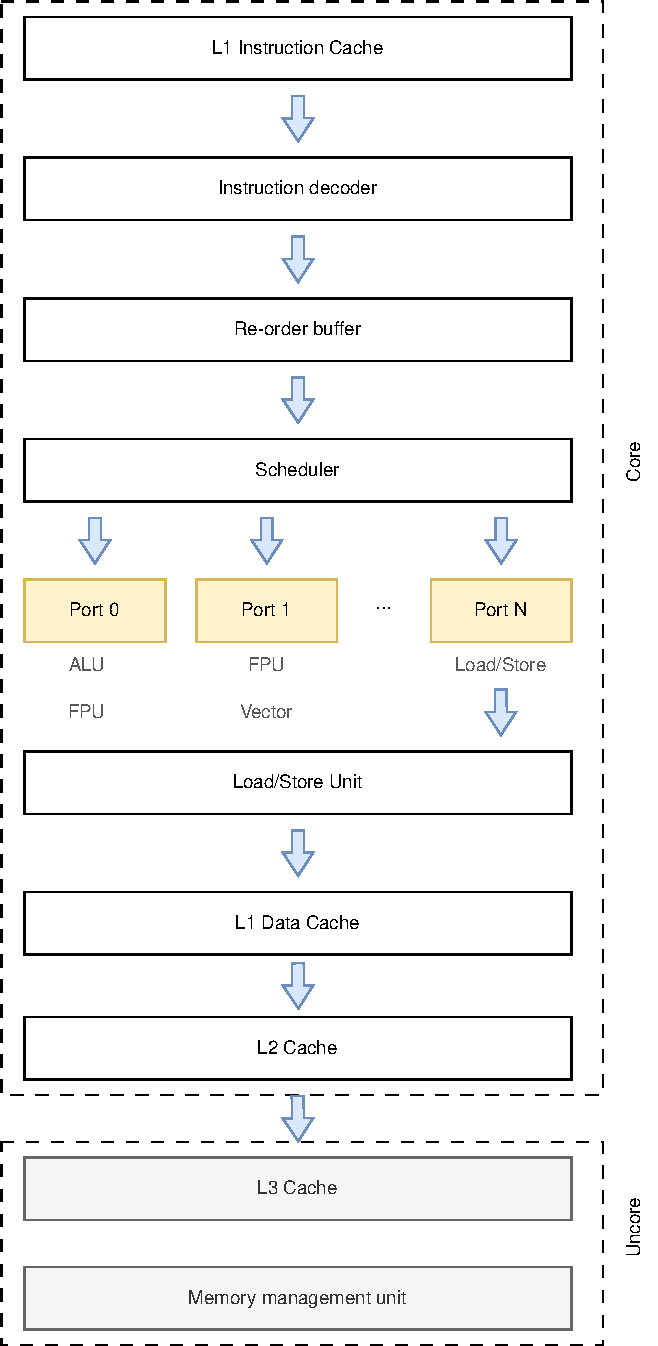
\includegraphics[scale=0.5]{cpu_uarch.pdf}
%   \centering
%   \caption{A typical modern CPU microarchitecture}
% \end{figure}

\subsection{Automatic basic block throughput measurement}

Profiling arbitrary basic blocks poses significant challenges. Memory access within a basic block often 
leads to segmentation faults. Yishen Chen et al. \cite{chenBHiveBenchmarkSuite2019} present a novel 
approach to deal with load or store instructions. They use process monitoring capabilities of the modern 
operating systems and map physical memory pages onto a virtual address space to avoid segmentation faults. 
Our methodology builds on this foundation, integrating LLVM target information to ensure portability 
across diverse platforms.

\subsection{Dataset construction and analysis}

Our toolkit's final component is dedicated to dataset construction, comprising two main programs. 
The first program processes text assembly files, converting them into a graph-based representation 
suitable for deep neural networks like LSTM or GNNs. We refer to these graphs as embeddings. 
The second program integrates embeddings with measurement results to produce a comprehensive dataset. 
Additionally, we offer a Python library to facilitate data analysis and ensure compatibility with 
platforms like Pytorch.

\subsection{Related work}

The landscape of microbenchmarking and performance modeling for modern CPU microarchitectures has 
seen significant advancements in recent years. A variety of approaches have been proposed to address 
the challenges in accurately estimating the performance of basic blocks.

One notable contribution is BHive, a benchmark suite and measurement framework designed specifically 
for validating x86-64 basic block performance models \cite{chenBHiveBenchmarkSuite2019}. Existing 
benchmark suites often focus on application-level performance and are not tailored for low-level 
basic block performance. BHive addresses this gap by providing a comprehensive set of basic blocks 
that are representative of real-world applications. Additionally, it includes tools for automated 
measurement and validation, facilitating the comparison of different performance models.

Focusing on recent Intel microarchitectures, uiCA presents a methodology that combines static analysis
and machine learning techniques for accurate throughput prediction of basic 
blocks \cite{abelUiCAAccurateThroughput2022}. Unlike approaches that aim for broad applicability, 
uiCA is optimized for high accuracy specifically on Intel CPUs. The authors demonstrate that their 
methodology outperforms existing methods, particularly for complex instruction sequences common in 
modern applications.

In contrast to traditional methods that rely on analytical models or table-based approaches, Ithemal 
introduces a deep learning-based model for estimating basic block throughput. Traditional methods 
often suffer from limitations such as inaccuracy or lack of portability across different microarchitectures.
Ithemal addresses these issues by employing a deep neural network trained on a large dataset of basic
blocks and their corresponding throughput values, measured on real hardware. This approach achieves high 
accuracy and is portable across different CPU architectures.

Kerncraft introduces an analytic performance modeling tool aimed at loop 
kernels \cite{hammerKerncraftToolAnalytic2017}. The paper presents a tool that utilizes a roofline model 
to predict the performance of loop kernels on various CPU architectures. Kerncraft aims to provide insights
into the performance bottlenecks and optimization opportunities for these critical sections of code.

Automated Instruction Stream Throughput Prediction presents a Open Source Architecture Code Analyzer, 
a static analysis tool for predicting the execution time of sequential loops comprising x86 instructions
under the assumption of an infinite first-level cache and perfect out-of-order 
scheduling \cite{laukemannAutomatedInstructionStream2018}. The paper introduces a machine model, tailored 
for modern Intel and AMD microarchitectures by semi-automated benchmarking.

Another tool that merits attention in the context of microbenchmarking and performance modeling is 
LLVM-Exegesis\footnote{\url{https://llvm.org/docs/CommandGuide/llvm-exegesis.html}}.
This tool is part of the LLVM compiler infrastructure and aims to 
empirically measure the latency and throughput of individual instructions on various CPU architectures. 
It generates microbenchmarks for specific instruction sequences and executes them to gather performance 
data. This empirical approach ensures high accuracy but is limited to the hardware on which the measurements
are taken. It serves as a valuable resource for compiler optimization and can be complementary to other 
methods that focus on predictive modeling.

While the existing tools and approaches set the foundation for in-depth performance analysis of assembly
code, they have some limitations in production applications. Specifically, these solutions are usually
constrained to specific architectures or microarchitectures. Our work is aimed at bridging some of
these gaps by providing a core infrastructure for automated benchmarking and processing of assembly
basic blocks, based on open-source LLVM framework and public OS interfaces.

\subsection{Contribution}

In this work we present an automatic assembly basic block dataset collection tool. Specifically, we make 
the following contributions:
\begin{itemize}
  \item \textit{An LLVM-based tool for basic block extraction, which automatically transforms binaries into a set 
        of assembly files}. This tool also performs basic filtering tasks, such as removing \textit{nop} 
        padding or excluding basic blocks with no meaningful computation.
  \item \textit{A profiling tool capable of benchmarking across multiple architectures.} We demonstrate how to utilize
        existing tools for benchmarking any basic block, ensuring minimal measurement variance. Practical 
        guidelines for setting up the profiling environment are also provided.
  \item \textit{A dataset construction tool that employs LLVM to assess basic block dependencies, converting the 
        data into a graph format.} This dataset paves the way for the development of deep learning cost 
        models utilizing Graph Neural Networks.
\end{itemize}

Figure \ref{fig:workflow} shows a complete workflow for the proposed toolkit.

\begin{figure*}[h]
  \centering
  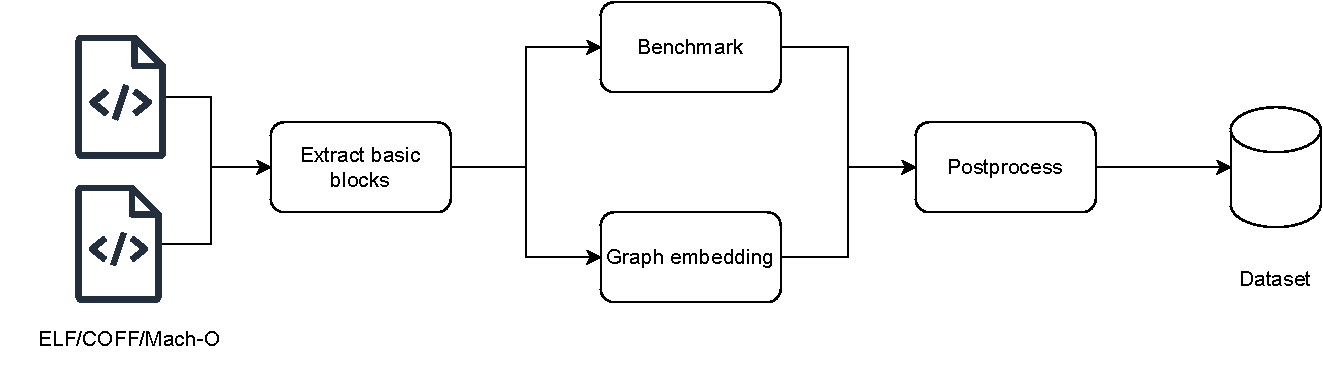
\includegraphics[width=0.8\linewidth]{workflow}
  \caption{Complete toolkit workflow}
  \label{fig:workflow}
\end{figure*}

Our toolkit is open-source and available online\footnote{\selflink{\url{https://github.com/perf-toolbox/llvm-ml}}}.

\section{Basic block extraction}

To provide accurate measurements of instruction latencies one must first prepare input data. There are 
two primary approaches for doing that: generating an artificial dataset and extracting basic blocks from
real-world programs.

\subsection{Basic block generation}

The first approach is taken by \textit{llmv-exegesis} tool. For each instruction in the ISA it can 
generate multiple samples of assembly. Those are usually different by the generation strategy. 
Modern desktop CPUs often employ out-of-order execution and pipelining, which allows them to execute 
multiple instructions at once, possibly, not in the order that these instructions are written in the 
code. In practice, that means that the CPU pipeline will have a register renaming unit, re-order buffer, 
and a scheduler, that can take an instruction from that buffer and dispatch it into a free port.

While such an optimization can greatly improve the performance of applications, it adds to the complexity 
of instruction benchmarking. The \textit{llvm-exegesis} tool can either generate a so-called "parallel" snippet, 
that can be used to estimate the number of available ports on the system, or a "serial" snippet, 
that can be used to measure a single instruction latency. The serialization is achieved by redirecting 
the output of the instruction to it's input and running that instruction in a loop. These two 
methodologies allow one to accurately describe some of the features of modern CPU architectures. 
This data is used by \textit{llvm-mca} and LLVM compiler stack to drive some of its cost models. 
A similar approach is taken by PMEvo tool, which can discover instruction port mapping using genetic 
algorithms \cite{ritterPMEvoPortableInference2020}. However, as shown by later research, these artificial 
basic blocks do not allow researchers to reveal some of the more sophisticated optimizations, like macro 
and micro fusion. Yishen Chen et al. \cite{chenBHiveBenchmarkSuite2019} have provided an estimation of 
the \textit{llvm-mca} tool relative error. Given a measured throughput $t$ and estimated throughput $t'$ a 
relative error is defined as $\operatorname{err}(t, t') = \frac{|t - t'|}{t}$. For \textit{llvm-mca} it has been found 
that the maximum relative error value is 0.54, which means that in worst-case scenario the estimation can
be off by 54\%, which in turn can lead to a wrong decision being made by the compiler backend.

\subsection{Dynamic extraction}

Another approach, that is often used is extracting basic blocks from compiled binaries. A typical 
approach would be to use a dynamic binary instrumentation tool to trace the actual execution of the 
instructions. This is how Mendis et al. collect the dataset for training 
Ithemal \cite{mendisIthemalAccuratePortable2019}.

These tools usually work by combining both disassembler and JIT compiler technology. For example, 
DynamoRIO uses five-level intermediate representations to process disassembled basic blocks:
\begin{itemize}
	\item \textbf{Level 0} is the raw instruction byte stream.
	\item \textbf{Level 1} is instructions stored as encoded bytes.
	\item \textbf{Level 2} is instructions decoded enough to determine their opcode.
	\item \textbf{Level 3} is fully-decoded instructions.
	\item \textbf{Level 4} is fully-decoded instructions that have been modified.
\end{itemize}
DynamoRIO then re-compiles these basic blocks and executes them natively. At the end of each basic 
block a so-called \textit{context switch} happens, and DynamoRIO takes control back to determine and 
prepare the next piece of executable.

The benefits of dynamic basic block extraction is that it allows one to extract data in the same form as 
CPUs see these instruction streams. Any branch that has not been taken during application execution 
will not be added to the final dataset. This can be useful for binaries that contain hand-optimized 
pieces of code or dynamically dispatched functions for uncommon ISA extensions.

The downside of dynamic approach is slow performance of this method. In practice, these tools still 
perform disassembling, but they also require users to run heavy workloads with additional tooling 
overhead. Furthermore, these tools aren't always available for target platforms.

\subsection{Static extraction}

As an alternative for dynamic extraction, we propose to use LLVM built-in Target framework to 
disassemble binaries and perform static analysis to clean up the data. To do so, we use the standard 
LLVM disassembly interface, iterating over sections of the given binary and trying to decode every 
instruction. We analyze each instruction in an online fashion. So-called \textit{nop} instructions are skipped 
at this stage. When disassembler meets a block terminator instruction, such as jump, call, system 
call, or return, it flushes all previously disassembled instructions into an assembly text file, 
clears the temporary buffer and increments basic block counter. After all sections are processed, 
the tool performs post-processing stage. During this stage, all recorded assembly files are parsed, 
and broken files are removed. The tool also removes all files, that only contain a single instruction, 
all files that only contain loads or stores, and all files that contain variable latency instructions. 
Single-instruction basic blocks are not representative for the purpose of CPU scheduler modeling. 
This kind of basic blocks is better synthesized in a controlled fashion to uncover some instruction 
properties, that are hard to infer with this kind of inputs. Memory processing-only basic blocks are 
removed since modern CPUs can perform various kinds of optimizations, like move 
elimination \cite{Intel64IA322022}, and thus are not representative either. Last, variable latency 
instructions are also hard to accurately model. Instructions, such as division or square root, may 
use iterative algorithms to compute the result value, and thus their latency fully depends on the 
value residing in the input register. The toolkit also removes duplicates by converting all basic 
blocks into graph representation and removing identical graphs. This allows us to also account for 
similar basic blocks where automatic register allocation algorithms worked slightly differently. 
While the graph representation also allows us to remove isomorphic graphs, we're not doing that on purpose. 
A different order of instructions may lead to different optimizations being triggered in the CPU pipeline 
even though two code pieces may be functionally identical.

\section{Profiling methodology}

\subsection{Generating benchmark harness}

In the process of generating a benchmark harness, we leverage the LLVM framework to construct a target 
function using LLVM Intermediate Representation (IR), subsequently executing it through the ORC JIT API. 
Each target function is meticulously crafted, comprising a prologue, an unrolled basic block, and an 
epilogue. The prologue serves three essential purposes:

\begin{itemize}
	\item \textbf{Preserving Register States}: It ensures that the test function can appropriately return
	       control to the host process by saving the current register states.
	\item \textbf{Configuring the Stack Pointer}: It sets the stack pointer to a predetermined segment of
	       memory that we've allocated beforehand.
	\item \textbf{Initializing Registers}: The registers are filled with a predefined value, ensuring
	       consistency in the testing environment.
\end{itemize}

Generating a target function also demands attention to certain unique considerations:
\begin{itemize}
	\item \textbf{Handling special floating-point conditions}: Floating-point operations may exhibit slow behavior in cases of denormals, underflows, or overflows. To counter this, we configure the CPU to raise an exception if any of these conditions occur. For x86 platforms, this control is exerted through the \textit{MXCSR} register.
	\item \textbf{Managing unaligned memory access}: Unaligned memory access can affect performance, and the x86 platform provides the ability to disable this access for specific threads. This is achieved by manipulating the \textit{EFLAGS} register. Other architectures, like AArch64 or RISC-V, offer similar functionality but often require privileged access. Such manipulation may impact both kernel and user code, potentially resulting in kernel panic during testing. An alternative approach is to either monitor a specialized PMU counter or apply a dynamic instrumentation technique to detect any unaligned access within a basic block during the test run.
\end{itemize}

Below is a piece of assembly code illustrating configuration of \textit{EFLAGS} register.

\begin{lstlisting}
add $-128, %rsp
pushf
orl $0x40000, (%rsp)
popf
sub $-128, %rsp
\end{lstlisting}

\subsection{Arbitrary basic block execution}

A fundamental obstacle in arbitrary basic block profiling is the handling of memory accesses, specifically 
those related to unallocated memory, which can lead to process crashes. To address this issue, we adopt 
the algorithm delineated by Chen et al. \cite{chenBHiveBenchmarkSuite2019}.

The process begins with a test run of the target basic block prior to the initiation of the profiling 
procedure. Should the process crash during this phase, the fault memory address is captured and added to 
a specific list. Subsequently, the process is restarted, and the aforementioned list is conveyed as an 
argument.

Utilizing \textit{mmap}, the process maps four memory pages to every address contained within the list. 
If a single instruction fails to access memory on two distinct occasions, the entire basic block is 
considered defective, causing the profiler to terminate its operation. The selection of four pages aims 
to preclude page aliasing, which has the potential to induce instruction serialization. This could occur 
despite the CPU's capability to execute the instructions in parallel. Although this phenomenon may also 
be observed in real software, performance estimation tools generally operate on idealized chip models 
that presuppose maximum parallelism.

Simultaneously, with a standard page size of 4 KiB, the allocation of four pages of memory should fit 
the L1 CPU cache appropriately. Refer to table \ref{tab:caches} to see the comparison of page size and 
L1 cache for modern architectures.

\begin{table*}[!t]
        \renewcommand{\arraystretch}{1.3}
        \caption{A comparison of modern CPU microarchitectures cache size}
        \centering
	\begin{tabular}{lllrrrr}
	        \hline
		CPU name      & Manufacturer & ISA     & L1 Data cache, KB                        & L1 Instruction cache, KB & L2 cache, MB & L3 cache, MB \\
		\hline
		EPYC 9354P    & AMD          & x86\_64 & 32                                       & 32                       & 32           & 256          \\
		Ryzen 9 7950X & AMD          & x86\_64 & 32                                       & 32                       & 16           & 64           \\
		Ryzen 5 3600  & AMD          & x86\_64 & 32                                       & 32                       & 3            & 32           \\
		i9-13900K     & Intel        & x86\_64 & 48                                       & 32                       & 2            & 36           \\
		GH200         & NVIDIA       & AArch64 & 64                                       & 64                       & 1            & 117          \\
		JH7110        & StarFive     & RISC-V  & 32                                       & 32                       & 2            & N/A
	\end{tabular}
        \label{tab:caches}
\end{table*}

\subsection{Profiling methodology}

Extracting timing information from modern superscalar pipelined architectures presents unique difficulties.
Most contemporary CPUs are equipped with a Performance Monitoring Unit (PMU) comprising specialized registers
and counters. These counters increment with each event occurrence and often encompass metrics such as the 
number of elapsed cycles, retired instructions, cache hits or misses, and more. Despite these capabilities, 
precisely mapping an event to a specific instruction proves challenging, since today's CPUs can decode, 
dispatch, and retire several instructions per cycle. Certain specialized hardware, such as Intel PEBS or 
AMD IBS, aims to address this challenge, but such features remain scarce, with very few chips offering this 
functionality \cite{bakhvalovPerformanceAnalysisTuning2020}.

To overcome these limitations, we employ a formula suggested by Abel and Reineke \cite{abelUiCAAccurateThroughput2022}:
\begin{equation}
\operatorname{throughput}(b) \approx \frac{\operatorname{cycles}(b, n) - \operatorname{cycles}(b, n')}{n - n'},
  \label{eq:throughput}
\end{equation}
where $\operatorname{cycles}(b, n)$ is the number of CPU cycles elapsed for a basic block unrolled with a factor of $n$,
and $n < n'$. Essentially, we execute two sets of benchmark harnesses and calculate the difference between
them. In this context, we refer to the shorter harness as noise and the longer one as workload. The value $n'$
is fixed and defined by user input, while $n$ is either fixed or dynamically determined by running noise
harness and measuring its time $t$ in nanoseconds. $n = \operatorname{min}(0.8 \times \frac{1000000 \times n'}{t}, \mathrm{MaxN})$.

This approach helps avoid L1 instruction cache misses by limiting the maximum number of iterations and 
dynamically reducing execution time for larger basic blocks. The constant $1'000'000$ is chosen as a 
conservative estimation of a time slice in nanoseconds, that an OS allocates to the thread. This number 
was chosen in assumption that the host OS employs completely fair scheduling mechanism. To make sure the 
benchmark gets as close to a full time slice as possible, we yield our thread right before running the 
harness.

In addition to the cycles counter, we collect the number of instructions retired, cache misses, and OS 
context switches. Accessing these counters is done through a library we wrote called 
\textit{libpmu}\footnote{\selflink{\url{https://github.com/perf-toolbox/libpmu}}}. 
Designed as a cross-platform tool, \textit{libpmu} interfaces with Performance Monitoring Units (PMUs) 
and even extends support to some unconventional architectures, such as SiFive's U74 core.

For each basic block, we perform $m$ runs for both the noise and workload harnesses. The instruction 
count should remain consistent across benchmark runs for the same number of basic block repetitions. 
If cache misses or context switches occur, the benchmark run is deemed a failure. If more than 10\% of 
runs in a batch fail, the entire basic block is discarded. We also compute the coefficient of variation 
for both workload batches, discarding the basic block if either exceeds 3\%.

Finally, we select the sample with the minimal number of elapsed cycles from both noise and workload 
batches, employing these values in formula \ref{eq:throughput}. By utilizing this refined approach, 
we strive to obtain more accurate timing information for modern CPU architectures, accommodating their 
complexities and optimizing performance analysis.

\subsection{Practical recommendations}

While conducting experiments, we identified several essential preconditions that must be fulfilled by 
the testing environment to guarantee stable and reliable results. These prerequisites revolve around 
system configurations to minimize variables that may introduce inconsistencies:

\begin{itemize}
	\item \textbf{Disabling Simultaneous Multiprocessing (SMT)}: Also known as Hyperthreading,
	       disabling this feature ensures that multiple threads do not run on the same physical
	       core simultaneously, thereby eliminating any interference. For Linux systems, this
	       can be achieved by appending the \textit{nosmt} flag during the kernel boot process.
	\item \textbf{Turning off frequency scaling and performance optimization features}: These
	       system configurations need to be disabled on the host CPUs to prevent automatic
	       adjustments that may skew results. By maintaining a constant frequency and eschewing
	       other optimization features, we can attain a more controlled and consistent testing environment.
	\item \textbf{Isolating CPU cores}: Isolation of CPU cores ensures that other processes
	       running on the system do not interfere with the core's L1 cache, either by flushing
	       or corrupting it. Our benchmarking tool is designed to bind the benchmark harness to
	       specific threads, defined by user input, thereby achieving precise control. For Linux
	       systems, core isolation can be implemented by passing the \textit{isolcpus=1,2,3,...,n}
	       flag during kernel boot.
\end{itemize}

These precautions serve to create a more uniform testing environment, minimizing the potential for 
extraneous factors to influence the outcome. By adhering to these guidelines, we strive to generate 
benchmark results that accurately reflect the performance characteristics under investigation.

\section{Dataset construction}

An assembly basic block dataset comprises two primary components: a graph-based representation of 
basic blocks and their associated throughput measurements.

\subsection{Graph-Based Representation of Basic Blocks}

In this graph representation, each assembly instruction within a basic block is encapsulated as a 
node. Edges between nodes signify data dependencies. The opcode for each instruction is stored as 
an attribute of the respective node. Additionally, our dataset construction utility captures a set 
of features for each instruction, such as whether it performs a memory load/store operation or vector 
arithmetic. The utility further offers the flexibility to introduce a virtual root node or to connect 
all nodes as a simple path, thereby enhancing compatibility with Graph Neural Networks (GNNs). Such 
a structure is advantageous since many GNN layers operate on the premise of message passing and require 
a connected graph to facilitate effective data flow. While other edges are usually present in the graph, 
incorporating a virtual root node can aid in interpreting instruction performance as it can interact with 
other instructions within the CPU's decoder or scheduler, even when no direct dependencies are evident. 
If an instruction reads from and writes to the same register, a self-loop is added to the corresponding 
node. A pseudocode outlining this graph construction algorithm is presented in a subsequent section. 
We employ an adjacency list to store the graph.

\subsection{Throughput Metrics}

The metrics component encompasses an array of measurements collected during noise and workload runs, 
along with the computed cycle counts and the actual number of basic block repetitions. The number of 
cycles is calculated as
\[\mathrm{cycles} = \operatorname{min}(\mathrm{cycles}^{\mathrm{workload}}_i) - \operatorname{min}(\mathrm{cycles}^{\mathrm{noise}}_j) \quad ~\forall i, j,\] while the number of runs 
is derived as 
\begin{equation*}
\begin{split}
N_{\mathrm{runs}} = &\operatorname{runs}(\operatorname{argmin}(\mathrm{cycles}^{\mathrm{workload}}_i)) - \\
  &\quad \operatorname{runs}(\operatorname{argmin}(\mathrm{cycles}^{\mathrm{noise}}_j)) \quad ~\forall i, j.
\end{split}
\end{equation*}
Subsequently, the reciprocal throughput for the basic block can be computed as 
\[\mathrm{throughput} = \frac{\mathrm{cycles}}{N_{\mathrm{runs}}}.\]

\subsection{Data Storage and Language Bindings}

The entire dataset is serialized using the Cap'n'Proto format\footnote{\url{https://capnproto.org/}},
allowing for language-agnostic usage. To further facilitate use of the dataset, we provide bindings for
both C++ and Python, thereby ensuring seamless integration with popular deep learning frameworks. Figure
\ref{fig:datastruct} shows the data structures employed to encapsulate the graph, measurements, and the
complete dataset.

\begin{figure}[h]
  \centering
  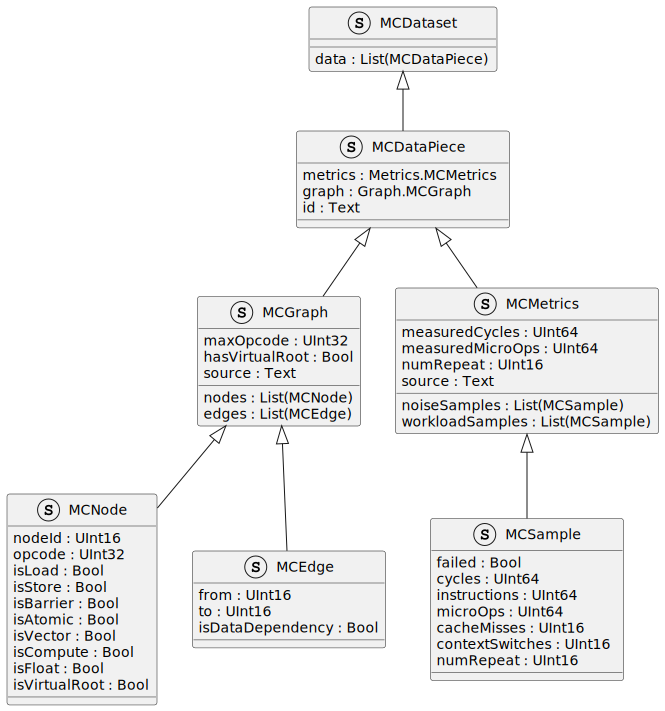
\includegraphics[width=0.9\columnwidth]{data_structures}
  \caption{Data structures used by the dataset construction tool}
  \label{fig:datastruct}
\end{figure}

\section{Evaluation}

The purpose of evaluation is to assess the accuracy and functional correctness of the proposed toolkit.
We also compare the collected data against \textit{llvm-mca} static estimations.

\subsection{Dataset and methodology}
We collect samples from various workloads and measure basic block latency using a benchmarking tool.
The metrics for evaluation include the mean absolute error (MAE) and the coefficient of variation.

For evaluation, we collect samples for the following workloads: x264 video codec, Clang compiler, 
Firefox browser's libxul library, and OpenBLAS library. The details about the initial dataset are 
shown in Table \ref{tab:test_data}.

\begin{table}[htbp]
  \caption{Overview of test data}
  \label{tab:test_data}
  \begin{tabular}{lrrr}
  \hline
  Workload & \# of basic blocks & \# measured & \# filtered \\
  \hline
  x264     & $80939$              & $44388$       & $30220$       \\
  libxul   & $436629$             & $213733$      & $158205$      \\
  Clang    & $365343$             & $195410$      & $143043$      \\
  OpenBLAS & $54865$              & $25302$       & $19673$       \\
  Total    & $937776$             & $478833$      & $351141$
  \end{tabular}
\end{table}

We use AMD Ryzen 5 3600 CPU for measurements and capture basic block throughput
estimations from the \textit{llvm-mca} tool.

\subsection{Results and discussion}
Figure \ref{fig:cov} shows the distribution of the coefficient of variation for
the measured data. Figure \ref{fig:lift_chart} shows the lift chart for measured
throughput values compared to \textit{llvm-mca} estimations. The MAE for this
experiment was $1.67$, while the mean measured latency was $3.85$. The mean relative
error was $0.34$. This means that on average the \textit{llvm-mca} tool is off by 34\%.
However, in the worst case scenario we've seen a maximum relative error of $24.4$.
Such a big error can be partially explained by a lower level of support for Zen 2
microarchitecture in LLVM CPU model.

\begin{figure}[h]
  \centering
  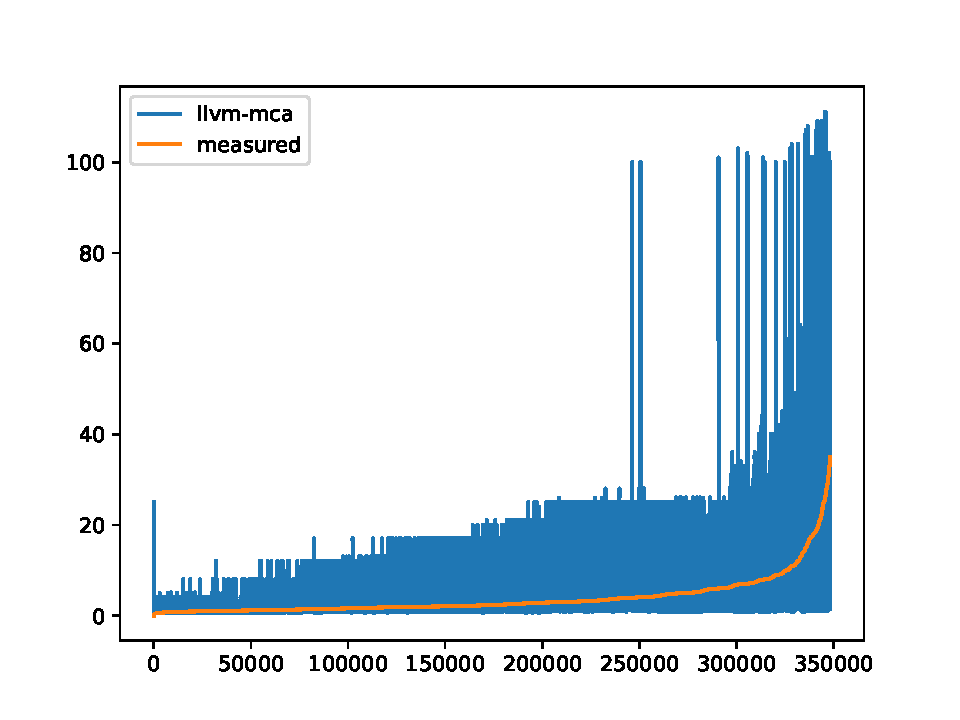
\includegraphics[width=0.9\columnwidth]{lift_chart_35_cycles}
  \caption{Lift chart for measured values vs \textit{llvm-mca} estimations capped at 35 cycles per basic block}
  \label{fig:lift_chart}
\end{figure}

\begin{figure}[h]
  \centering
  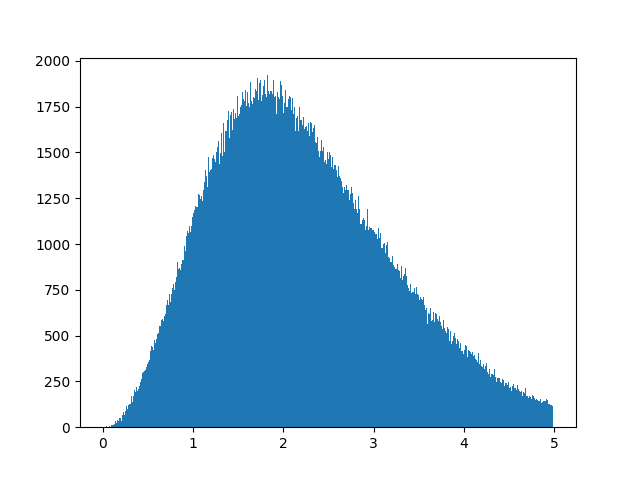
\includegraphics[width=0.9\columnwidth]{cov_distribution_zoom}
  \caption{Distribution of coefficient of variation for unfiltered data capped at 5\%}
  \label{fig:cov}
\end{figure}

An example of mispredicted basic blocks can be found in Appendix \ref{appendix:listings}.
Both examples have been found in the Clang compiler binary code. Measured throughputs for these
examples are $3.5$ and $3.35$, and the estimation was $25.04$ and $25.03$ respectively, which
corresponds to relative error values $6.15$ and $6.47$. We also run estimations for Intel Cascade Lake,
Ice Lake, Tiger Lake, and Rocket Lake, and the values on all platfroms are $37.04$ and $37.03$ respectively
for both basic blocks. These examples show that \textit{llvm-mca} particularly struggles with stack instruction
optimizations happening inside a processor core. The exact reasons behind this behavior of the model are
yet to be discovered.

Finally, we build a graph representation for each basic block in the dataset. 
Figure \ref{fig:sample_graph} shows an example of such a graph for a basic block snippet below.
In this representation the information about particular registers is lost. That is consistent
with how compilers (such as LLVM) internally represent code in pre-register allocation stages.

\begin{lstlisting}[title={Source of the sample basic block}]
movq	%rdi, 16(%rsp)
addq	$8, %rdi
movq	%rdi, 56(%rsp)
movq	%r14, %rsi
movl	%edx, 32(%rsp)
movl	$1, %ecx
\end{lstlisting}

\begin{figure}[h]
  \centering
  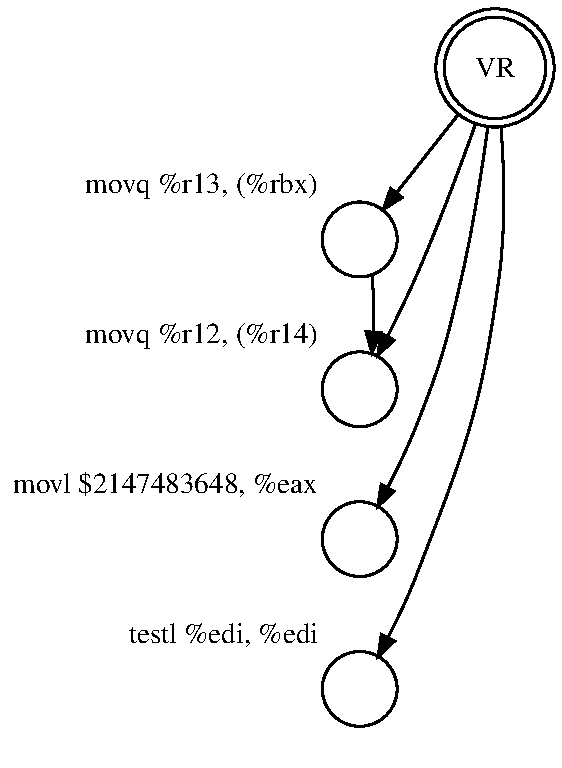
\includegraphics[width=0.4\columnwidth]{sample_graph}
  \caption{Sample basic block graph. Source of origin: \textit{libxul}. Measured cycles: 1.95.}
  \label{fig:sample_graph}
\end{figure}

\section{Conclusion and future work}

Performance modeling is a cornerstone for optimizing compilers, yet existing models often 
fall short in terms of accuracy and applicability across diverse architectures. This paper 
has introduced an automated toolkit aimed at addressing these limitations. Our LLVM-based 
approach for basic block extraction offers a more versatile and efficient alternative to existing 
microbenchmarking tools, thereby expanding the scope of platforms that can be profiled and evaluated. 

Our profiling tool builds upon existing methodologies to offer a robust and portable solution for 
benchmarking of basic blocks. This tool is designed to minimize measurement variance, thereby 
increasing the reliability of the collected data. Furthermore, we have developed a dataset construction 
tool that transforms basic blocks into graph-based representations, laying the groundwork for future 
research in deep learning-based cost models.

Our contributions are threefold:
\begin{itemize}
    \item We provide an LLVM-based tool for efficient and versatile basic block extraction.
    \item We introduce a robust profiling tool capable of benchmarking across multiple architectures.
    \item We offer a dataset construction tool that enables the development of advanced cost models based on Graph Neural Networks.
\end{itemize}

We see the following ways for future work:
\begin{itemize}
  \item Expand benchmarking tool to other CPU platforms. We used LLVM as a foundation for our 
    toolkit and Linux \textit{perf} APIs to collect performance data, meaning that adding a new CPU
        platform is a logical next step.
  \item Expand benchmarking tool to accelerator platforms, such as GPUs. The CPU benchmarking tool
        heavily relies on memory mapping capabilities. Modern discrete GPUs also provide such a capability,
        meaning that it is possible to use the same technique (with slight modifications) to perform benchmarking.
  \item Building a deep learning-based model for static performance evaluation of the arbitrary code.
\end{itemize}
